\documentclass[11pt]{article}
\usepackage[T1]{fontenc}
\usepackage[utf8]{inputenc}
\usepackage{lmodern}
\usepackage[margin=1in]{geometry}
\usepackage{amsmath,amssymb,amsthm,mathtools}
\def\DoNotLoadEpstopdf{}
\usepackage{tikz}
\usepackage{float}
\usepackage{microtype}
\usepackage[colorlinks=true,linkcolor=blue!45!black,citecolor=blue!45!black,urlcolor=blue!45!black]{hyperref}
\usepackage{bookmark}
\hypersetup{pdfauthor={OpenAI},pdftitle={Asymptotically minimal maxima of real Littlewood polynomials}}
\newtheorem{theorem}{Theorem}[section]
\newtheorem{proposition}[theorem]{Proposition}
\newtheorem{lemma}[theorem]{Lemma}
\newtheorem{corollary}[theorem]{Corollary}
\theoremstyle{definition}
\newtheorem{definition}[theorem]{Definition}
\theoremstyle{remark}
\newtheorem{remark}[theorem]{Remark}
\newcommand{\T}{\mathbb T}
\newcommand{\R}{\mathbb R}
\newcommand{\Z}{\mathbb Z}
\newcommand{\N}{\mathbb N}
\newcommand{\C}{\mathbb C}
\newcommand{\e}{\mathrm e}
\newcommand{\norm}[1]{\left\lVert #1\right\rVert}
\DeclareMathOperator{\sgn}{sgn}
\title{Asymptotically minimal maxima of real Littlewood polynomials}
\author{OpenAI}
\date{September 23, 2026}
\begin{document}
\maketitle
\begin{abstract}
We prove that the minimum possible maximum modulus on the unit circle of a polynomial
with $N$ consecutive real coefficients in $\{-1,1\}$ is $(1+o(1))\sqrt N$,
as $N$ tends to infinity through all integers. This disproves the real-sign
analogue of Erd\H{o}s's fixed relative-gap conjecture. As a consequence,
the largest binary merit factor at length $N$ tends to infinity through all
integer lengths, disproving Turyn's conjecture.
\end{abstract}
\tableofcontents
\section{Introduction}\label{sec:introduction}
Write $\T=\R/\Z$ and $\e(t)=\exp(2\pi i t)$. All tori carry probability
Haar measure. A Littlewood polynomial of length $N$ is a polynomial
\[
 P(z)=\sum_{k=0}^{N-1}\varepsilon_k z^k,
 \qquad \varepsilon_k\in\{-1,1\}.
\]
Its maximum modulus is $\norm{P}_\infty=\max_{t\in\T}|P(\e(t))|$.
Define
\[
 m_N=\min_{\varepsilon_0,\ldots,\varepsilon_{N-1}\in\{-1,1\}}
       \frac{1}{\sqrt N}\norm{\sum_{k=0}^{N-1}\varepsilon_k z^k}_\infty.
\]
Orthogonality gives $\norm{P}_2^2=N$, so $m_N\ge1$. The real-sign
analogue of Erd\H{o}s's fixed-gap question asks whether $m_N$ is
eventually bounded below by $1+c$ for some absolute $c>0$.
Erd\H{o}s's original question allowed complex unimodular coefficients
and was refuted in that class by Kahane; the restriction to real signs
is the question addressed here \cite[Problem~22]{Erdos1957}; see also
\cite{Kahane1980} and \cite[Problems~4.13 and~4.31]{HaymanLingham2018}.

\begin{theorem}\label{thm:main}
For Littlewood polynomials with real coefficients,
\[
 \lim_{N\to\infty}m_N=1.
\]
Equivalently, for every $\eta>0$ there is $N_0$ such that for every integer
$N\ge N_0$ there are signs $\varepsilon_0,\ldots,\varepsilon_{N-1}$ with
\[
 \max_{|z|=1}\left|\sum_{k=0}^{N-1}\varepsilon_kz^k\right|
 \le(1+\eta)\sqrt N.
\]
\end{theorem}

The theorem concerns every sufficiently large length, rather than a
subsequence. It gives no uniform lower bound for $|P(z)|$ and hence does
not assert two-sided uniform ultraflatness. The choices in the proof are
existential; no useful convergence rate or efficient signing algorithm
is asserted.

\subsection{Context and comparison}
The Shapiro--Rudin construction, obtained earlier by Shapiro and
independently by Rudin, gives real-sign polynomials
with maximum $O(\sqrt N)$; at dyadic lengths its paired identity gives
an upper bound $\sqrt{2N}$ \cite[Theorem~I and its proof]{Rudin1959}.
Balister proved the
all-length bound $\sqrt{6N-2}-1$ for its initial segments
\cite[Theorem 1]{Balister2019}. A different problem asks for upper and
lower bounds by fixed positive multiples of $\sqrt N$ throughout the
circle. Such two-sided flat Littlewood polynomials were constructed by
Balister, Bollob\'as, Morris, Sahasrabudhe and Tiba, whose proof combines
the Shapiro--Rudin construction with discrepancy theory
\cite{BalisterEtAl2020}. These results control the scale of the maximum,
but do not make the upper constant tend to one.

The coefficient class matters. Complex coefficients of modulus one allow
ultraflat constructions. Littlewood used quadratic phases near this
Parseval scale, Kahane obtained ultraflatness, and Bombieri and Bourgain
gave quantitative constructions \cite{Littlewood1966,Kahane1980,BombieriBourgain2009}.
The smoothed quadratic phases and Poisson summation used in
\cite[Sections~2 and~7]{BombieriBourgain2009} are analytic predecessors
of the sampling argument below. Their bounded-to-unimodular correction
also develops a method of K\"orner
\cite[Section~8]{BombieriBourgain2009}. The present proof must instead
preserve real coefficients and round them to signs. The distinction
between the unimodular and real-sign questions is also explicit in
\cite[Problem 4.31]{HaymanLingham2018}.
Georgiev, G\'omez-Serrano, Tao and Wagner recently used AlphaEvolve to
search for the same real-sign minimum at degrees up to $100$;
their computations do not give an asymptotic theorem
\cite[Section 6.13]{GeorgievEtAl2025}.

There can still be a growing additive gap above Parseval's bound.
Erd\'elyi proved that every Littlewood polynomial of length $N$ satisfies
\cite[Theorem 2.1]{Erdelyi2026}
\[
 \norm{P}_\infty^2\ge N+\frac{(N-1)^{1/3}}{38}.
\]
The extra term divided by $N$ tends to zero, so this is compatible with
Theorem~\ref{thm:main}.

The theorem implies flatness in every fixed finite $L^p$ modulus
sense. This conflicts with nonflatness claims in preprints of
el Abdalaoui \cite{ElAbdalaoui2017,ElAbdalaoui2025,ElAbdalaoui2025Generalization}.
Section~\ref{sec:finite-flatness} proves the implication with our
normalization. Appendix~\ref{sec:concentration} examines specific issues in
the contrary arguments.

\subsection{Merit factors and a symbolic spectral consequence}
For a binary word $A=(a_0,\ldots,a_{N-1})\in\{-1,1\}^N$ of length
$N\ge2$, define its aperiodic sidelobe autocorrelations and merit factor by
\[
 C_u(A)=\sum_{j=0}^{N-1-u}a_ja_{j+u}\quad(1\le u<N),
 \qquad
 F(A)=\frac{N^2}{2\sum_{u=1}^{N-1}C_u(A)^2}.
\]
This is the standard merit-factor normalization
\cite[Definition~2 and Lemma~0]{DownarowiczLacroix1998}; see also
\cite[Introduction]{JedwabKatzSchmidt2013} for its fourth-moment formulation.
The conjectured boundedness of $F(A)$ over all such words is called
Turyn's conjecture, equivalently Erd\H{o}s's $L^4$-norm conjecture, in
\cite[p.~3 of the author manuscript]{DownarowiczLacroix1998}.
For comparison, Jedwab, Katz and Schmidt constructed families with
limiting merit factor $6.342061\ldots$, improving the
previous proven value $6$, by modifying and extending Legendre sequences
\cite[Theorem~1.1 and Corollary~3.2]{JedwabKatzSchmidt2013}.
Section~\ref{sec:merit-morse} disproves this boundedness in the stronger
all-length form: the largest merit factor at length $N$ tends to infinity
as $N$ tends to infinity through all integers.

Downarowicz and Lacroix also relate this question to binary Morse shifts,
the discrete-time symbolic systems generated by iterated products of binary
words. Their theorem converts unbounded binary merit factors into a uniquely
ergodic binary Morse shift with simple spectrum whose zero-coordinate
spectral measure is absolutely continuous with an $L^2$ density
\cite[Theorem~2 and its proof]{DownarowiczLacroix1998}.
Section~\ref{sec:merit-morse} gives the precise spectral statement and its
deduction from Theorem~\ref{thm:main}.

\subsection{Proof overview}
We first allow real coefficients $X_{N,k}\in[-1,1]$. Their defect from
being signs is measured by
\[
 \mu(X_N)=\frac12\sum_{k=0}^{N-1}(1-|X_{N,k}|).
\]
The construction makes the normalized Fourier maximum close to one
while keeping $N^{-1}\sum_k X_{N,k}^2$ close to one. The latter condition
makes $\mu(X_N)/N$ small. A discrepancy argument then replaces the
coefficients by signs, with an error controlled by this small defect.
Section~\ref{sec:reduction} states both intermediate results precisely
and gives the deduction of the theorem.

To build the relaxed coefficients, we use a real trigonometric polynomial
$F$ on an auxiliary torus whose absolute value is at most one and whose
mean-square mass is nearly one. Each Fourier mode of $F$ is assigned a
nonzero quadratic curvature. A stationary-phase calculation shows that
sampling such a mode on a block spreads its Fourier contribution over
an interval whose width is proportional to that curvature. There are two
requirements: distinct modes and blocks must have disjoint intervals,
and each individual contribution must have size at most approximately
$\sqrt N$.

Section~\ref{sec:packing} supplies the interval packing, even when the
integer frequency vectors have linear relations. It uses a randomly
constructed finite-field hypergraph and the Pippenger--Spencer coloring
theorem, in the near-perfect-packing lineage of Frankl and R\"odl
\cite{FranklRodl1985,PippengerSpencer1989,AlonYuster2005}.
Section~\ref{sec:spreading} adjusts the Fourier coefficients of $F$ by
quadratic oscillations in extra variables so that their sizes match the
available widths. Section~\ref{sec:sampling} samples the resulting fixed
polynomial on disjoint blocks. At each angle at most one stationary
contribution remains, whereas orthogonality in the sampling limit
recovers nearly full mean-square mass.

Finally, Section~\ref{sec:rounding} proves the defect-sensitive rounding
bound. We use the partial-coloring method of Beck and Spencer
\cite{Beck1981,Spencer1985}, in the arbitrary-vector form verified through
Lovett--Meka's theorem \cite{LovettMeka2015}. A dyadic rounding procedure
keeps the defect mass from increasing, which makes its total loss
$o(\sqrt N)$ as the target error decreases. All auxiliary dimensions,
frequencies, primes, blocks and smooth cutoffs are fixed before $N$
tends to infinity.

\section{Reduction to approximation and rounding}\label{sec:reduction}
For a vector $X=(X_0,\ldots,X_{N-1})\in[-1,1]^N$, write
\[
 Q_X(t)=\sum_{k=0}^{N-1}X_k\e(kt),\qquad
 \mu(X)=\frac12\sum_{k=0}^{N-1}(1-|X_k|).
\]
The first proposition constructs vectors with small Fourier maximum and
nearly maximal energy. Its proof occupies Sections~\ref{sec:packing}--\ref{sec:sampling}.

\begin{proposition}[Almost-sign approximation]\label{prop:almost-signs}
For every $0<\delta<1/20$, there are vectors
$X_N=(X_{N,0},\ldots,X_{N,N-1})\in[-1,1]^N$, one for each integer
$N\ge1$, such that
\begin{align}
 \limsup_{N\to\infty}\frac{\norm{Q_{X_N}}_\infty}{\sqrt N}
 &\le K_\delta,
 &K_\delta&=\sqrt{\frac{(1+\delta)^3}{1-\delta}},
 \label{eq:almost-maximum}\\
 \liminf_{N\to\infty}\frac1N\sum_{k=0}^{N-1}X_{N,k}^2
 &\ge1-7\delta.\label{eq:almost-energy}
\end{align}
\end{proposition}

The next lemma converts an arbitrary relaxed vector to signs. Its
constant does not depend on the vector or its length. We prove it in
Section~\ref{sec:rounding}.

\begin{lemma}[Rounding with a small defect]\label{lem:rounding}
There is an absolute constant $C$ such that for every $N\ge1$ and every
$X\in[-1,1]^N$, some signs $\varepsilon_0,\ldots,\varepsilon_{N-1}$
satisfy
\begin{equation}\label{eq:defect-rounding}
 \max_{t\in\T}\left|\sum_{k=0}^{N-1}(\varepsilon_k-X_k)\e(kt)\right|
 \le C\left(1+\sqrt{\mu(X)\log\frac{80N}{\mu(X)}}\right).
\end{equation}
The square-root term is defined to be zero when $\mu(X)=0$; in that case
$X$ already has sign entries and the left side may be zero.
\end{lemma}

\begin{proof}[Proof of Theorem~\ref{thm:main}]
Fix $0<\delta<1/20$ and choose the family from
Proposition~\ref{prop:almost-signs}. For all sufficiently large $N$,
\eqref{eq:almost-energy} gives
\[
 \frac1N\sum_kX_{N,k}^2\ge1-8\delta.
\]
Since $1-|x|\le1-x^2$ for $|x|\le1$, it follows that
$\mu(X_N)\le4\delta N$. The function
$u\mapsto u\log(80N/u)$ is increasing on $0<u\le N/2$.
Applying Lemma~\ref{lem:rounding} and then
\eqref{eq:almost-maximum}, we obtain
\[
 \limsup_{N\to\infty}m_N
 \le K_\delta+2C\sqrt{\delta\log(20/\delta)}.
\]
First the limit in $N$ was taken with every auxiliary choice depending
on $\delta$ fixed. Now let $\delta\downarrow0$. The right side tends to
one, and the lower bound $m_N\ge1$ follows from Parseval. This proves
the limit through all positive integer lengths.
\end{proof}

\section{Packing signed intervals}
\label{sec:packing}

The sampling construction will divide the coefficient positions into
$H$ blocks, each of normalized length $1/H$. To explain the packing
required, consider one mode with coefficient $c\in\C$, a smooth cutoff
$0\le\chi\le1$ supported strictly inside its block, linear frequency
$\eta\in\R$, and nonzero quadratic curvature $\lambda\in\R$ with
$|\lambda|/H<1$. On a block centered at $x_*$ its phase, with $x=k/N$, is
\[
 N\left(\frac{\lambda}{2}(x-x_*)^2+(t+\eta)x\right).
\]
After allowing for integer frequencies in Poisson summation, a stationary
point in the cutoff support can occur only when $-t$ belongs to the circle
interval centered at
$\eta\pmod1$ of width $|\lambda|/H$. With the mode and cutoff fixed,
quadratic stationary phase gives the asymptotic bound
$|c|/\sqrt{|\lambda|}$ for its contribution divided by $\sqrt N$.
We therefore reserve total width $|\lambda|$ across the $H$ blocks for
this mode, while each block has the same peak bound. Section~\ref{sec:sampling}
will make these estimates uniform in $t$. For a real auxiliary polynomial,
opposite Fourier modes produce opposite centers and equal widths, so both
intervals must be reserved.

We now prove the geometric statement needed to separate all these
stationary intervals. Their centers must be values of specified integer
linear forms at one common point for each block. We allow relations
among three or more forms; the only independence assumption concerns
pairs of forms.

For $\eta\in\T$ and $0<\ell<1$, write
\[
 I(\eta,\ell)=\{\eta+x\pmod 1:-\ell/2\le x\le\ell/2\}
\]
for the closed interval with center $\eta$ and length $\ell$.

\begin{lemma}[Signed interval packing]
\label{lem:signed-packing}
Let $m\ge1$ and $r\ge2$ be integers, and let $a_1,\ldots,a_r\in\Z^m\setminus\{0\}$
be pairwise nonparallel.  If $w_1,\ldots,w_r>0$ satisfy
$2\sum_iw_i<1$, there exist an integer $H\ge1$ and points
$\theta_1,\ldots,\theta_H\in\T^m$ such that the $2rH$ closed intervals
\[
 I\bigl(\sigma a_i\cdot\theta_h,w_i/H\bigr),
 \qquad 1\le i\le r,\quad 1\le h\le H,\quad \sigma\in\{-1,1\},
\]
are pairwise disjoint.
\end{lemma}

We will use the following form of the Pippenger--Spencer edge-coloring
theorem \cite{PippengerSpencer1989}; the quantified statement below is
\cite[Lemma~2.1]{AlonYuster2005}.  A hypergraph here is finite and has distinct edges,
each an $r$-element subset of its vertex set.  Its degree $d(v)$ counts
edges containing $v$, and its codegree $d(u,v)$ counts edges containing
both distinct vertices $u,v$.  An edge coloring partitions the edges
into matchings, where a matching is a collection of pairwise disjoint edges.

\begin{theorem}[Pippenger--Spencer]
\label{thm:packing-edge-coloring}
For each integer $r\ge2$ and each $\gamma>0$, there exists $\beta>0$
with the following property.  If an $r$-uniform hypergraph satisfies,
for some $t>0$,
\[
 (1-\beta)t<d(v)<(1+\beta)t\quad\text{for every vertex }v,
 \qquad d(u,v)<\beta t\quad\text{for }u\ne v,
\]
then its edges can be partitioned into at most $(1+\gamma)t$ matchings.
\end{theorem}

In particular, for fixed $r$, degrees $(1+o(1))D$ and maximum
codegree $o(D)$ give an edge coloring with $(1+o(1))D$ colors.
We construct such a hypergraph whose vertices are small disjoint slots
in a half-circle.  An edge records one compatible center of each type.
A large matching will provide many compatible choices without reusing
any slot.

\begin{proof}[Proof of Lemma~\ref{lem:signed-packing}]
All constants implicit in asymptotic estimates may depend on the fixed
forms and the fixed slot lengths chosen next.  The sole parameter tending
to infinity in this proof will be a prime $q$.

\paragraph{Slot lengths and finite-field ranks.}
Choose positive proportions $\alpha_i>2w_i$ with $\sum_i\alpha_i=1$.
Approximating $T\alpha_i$ by positive odd integers as $T\to\infty$
gives fixed odd integers $L_i$ such that, with $L=\sum_iL_i$,
\begin{equation}
 w_i<\frac{L_i}{2L}\qquad(1\le i\le r).
 \label{eq:packing-width-slack}
\end{equation}
Let $b$ be the rank over $\mathbb Q$ of the matrix whose rows are the $a_i$.
Then $b\ge2$.  For every sufficiently large prime $q$, the full matrix
has rank $b$ over $\mathbb F_q$, and each pair of rows has rank two.
Indeed, it suffices to exclude the prime divisors of a nonzero
$b$-by-$b$ minor and of one nonzero two-by-two minor for each pair.
Fix such a prime for the following construction.

\paragraph{Random slots and oriented centers.}
Put $n=(q-1)/2$, $R=\lfloor\sqrt q\rfloor$, and
$U_q=\{1,\ldots,n\}$.  For $s\in\mathbb F_q$, let $|s|_q$
be the absolute value of its representative in $[-n,n]$.
Partition $U_q$ into consecutive chunks of $R$ sites, with a possible
final shorter chunk.  There are $K=\lceil n/R\rceil$ chunks.

Consider a periodic partition of the integers into consecutive slots:
each period has one slot of type $i$, consisting of $L_i$ consecutive
sites, for each $i=1,\ldots,r$.  Independently in each chunk, translate
this pattern by a uniform residue modulo $L$, and keep only slots
entirely contained in that chunk.  A kept slot is a vertex of its type.
Its middle site $c$ is an integer because $L_i$ is odd.  Give it an
oriented center $s=c$ or $s=-c$ in $\mathbb F_q$, with equal probabilities,
independently for all kept slots.  The random data in different chunks
are independent.

A chunk of length $u$ contains $u/L+O(1)$ kept slots of each type,
uniformly in its shift.  Thus in every realization the number of
vertices of each type is
\begin{equation}
 \frac nL+O(K)=\frac q{2L}+O(q/R+1).
 \label{eq:packing-vertex-count}
\end{equation}
This estimate includes the last short chunk.  Call a site interior if
its distance from both endpoints of its chunk is at least $L$.
For any nonzero $u\in\mathbb F_q$ whose folded site $|u|_q$ is interior,
the probability that $u$ is the oriented center of a vertex of a specified
type $j$ is exactly
\begin{equation}
 p=\frac1{2L}.
 \label{eq:packing-center-probability}
\end{equation}
There is exactly one shift modulo $L$ placing a type-$j$ middle site
there; the resulting slot is fully contained in the chunk, and its
orientation has the required sign with probability $1/2$.

\paragraph{Compatible tuples form a simple hypergraph.}
An edge is a tuple of one vertex of each type, with oriented centers
$s_1,\ldots,s_r$, for which the equations
\[
 a_i\cdot y=s_i\qquad(1\le i\le r)
\]
have a solution $y\in\mathbb F_q^m$.  We keep one edge per tuple,
regardless of the number of solutions.  Every compatible tuple has
exactly $q^{m-b}$ solutions, the size of the kernel of the rank-$b$
evaluation map.  This constructs a simple $r$-uniform hypergraph.

Write $C_j(u)$ for the indicator that $u$ is the oriented center of a
type-$j$ vertex.  For nonzero $s$, define the random variable
\[
 Z_{i,s}=\frac1{q^{m-1}}
 \sum_{\substack{y\in\mathbb F_q^m\\a_i\cdot y=s}}
       \prod_{j\ne i}C_j(a_j\cdot y).
\]
When the vertex of type $i$ with center $s$ exists, its degree is exactly
\begin{equation}
 d(i,s)=q^{b-1}Z_{i,s}.
 \label{eq:packing-degree}
\end{equation}
This follows by dividing the number $q^{m-1}Z_{i,s}$ of generating
vectors by $q^{m-b}$.  Likewise, two fixed evaluations of different
types leave $q^{m-2}$ possible vectors, so their codegree is at most
\begin{equation}
 q^{b-2}.
 \label{eq:packing-codegree}
\end{equation}
Two vertices of the same type have codegree zero.

We next show that nearly all vertices have nearly the same degree.
Although evaluations of several forms may be dependent, their folded
sites usually belong to different chunks.  The independent chunk
choices then supply the first and second moments we need.

\paragraph{Exceptional centers and the moment estimates.}
For a fixed type $i$, let $E_i$ contain those nonzero $s\in\mathbb F_q$
for which there exist $j<l$, both different from $i$, and a relation
\begin{equation}
 a_j+a_l=c a_i\quad\text{or}\quad a_j-a_l=c a_i,
 \qquad |cs|_q\le R.
 \label{eq:packing-exceptional-relation}
\end{equation}
Any such relation has a unique nonzero $c$: if $c=0$, the two forms
$a_j,a_l$ would be parallel over $\mathbb F_q$.  For each relation,
multiplication by $c$ is a bijection, so at most $2R+1$ residues are
excluded.  There are at most $2\binom{r-1}{2}$ relations, giving
\begin{equation}
 |E_i|=O(R).
 \label{eq:packing-exception-count}
\end{equation}

Fix a nonzero $s\notin E_i$, and sample $y$ uniformly on the affine fiber
$a_i\cdot y=s$.  Each other evaluation $a_j\cdot y$ is uniform on
$\mathbb F_q$, by pairwise rank two.  Let $Q_s$ be the chunk containing
$|s|_q$.  At most $2LK$ positive sites are noninterior; this bound also
covers a short final chunk with no interior sites.  Including their
negatives, zero, and the residues folding into $Q_s$, the probability
that a specified evaluation fails to fold into an interior site outside
$Q_s$ is at most
\[
 \tau_q=\frac{1+4LK+2R}{q}=O(q^{-1/2}).
\]

If two residues fold into one chunk, the difference of their folded
sites has absolute value at most $R$.  Consequently at least one of
their sum and difference has folded absolute value at most $R$.
For $a_j\cdot y$ and $a_l\cdot y$, each of these signed combinations
is either uniform on $\mathbb F_q$ under $a_i\cdot y=s$, or is the
constant $cs$ from a relation in
\eqref{eq:packing-exceptional-relation}.  The latter case cannot cause
a collision because $s\notin E_i$; the former has probability at most
$(2R+1)/q$.  Thus the $r-1$ evaluations fold into distinct interior
chunks different from $Q_s$, except on an $O(q^{-1/2})$ fraction of
the fiber.

For the second moment, take two independent uniform vectors $y,y'$
from the same fiber.  The preceding bounds apply within each copy.
Across copies, $a_j\cdot y$ and $a_l\cdot y'$ are independent uniform
residues for any $j,l\ne i$, including $j=l$; their sum and difference
are therefore uniform.  A union bound shows that the combined list
of $2(r-1)$ evaluations also occupies distinct interior chunks
outside $Q_s$, apart from a fraction $O(q^{-1/2})$.
More explicitly, for either $u=1$ or $u=2$ independent fiber samples,
the failure fraction is at most
\begin{equation}
 u(r-1)\tau_q+
 2\binom{u(r-1)}2\frac{2R+1}{q}=O(q^{-1/2}).
 \label{eq:packing-good-tuples}
\end{equation}
This bound uses no joint independence among the forms in one copy.

Let $V_{i,s}$ be the event $C_i(s)=1$, and condition on it whenever
it has positive probability.  The event depends only on random data
in $Q_s$.  Each tuple counted as good in
\eqref{eq:packing-good-tuples} uses distinct other chunks, where the
required center hits are independent and each has probability $p$.
The good-tuple condition itself depends only on the fiber vectors,
not on the slot choices.  Averaging over those vectors, and bounding
the contribution of bad tuples between zero and one, gives
\begin{align}
 \mathbb E[Z_{i,s}\mid V_{i,s}]&=p^{r-1}+O(q^{-1/2}),
 \label{eq:packing-first-moment}\\
 \mathbb E[Z_{i,s}^2\mid V_{i,s}]&=p^{2(r-1)}+O(q^{-1/2}).
 \label{eq:packing-second-moment}
\end{align}
The expectations are over the random slots and orientations.
The second identity follows by expanding the square as the average
over the independent pair $y,y'$.  Both error bounds are uniform in
nonexceptional $s$.  The conditioned vertex itself need not be
interior: avoiding its entire chunk makes that unnecessary.

\paragraph{Deleting the few vertices of atypical degree.}
Set $D_q=p^{r-1}q^{b-1}$ and $\varepsilon_q=q^{-1/8}$.
Equations~\eqref{eq:packing-first-moment}--\eqref{eq:packing-second-moment}
imply
\[
 \mathbb E\bigl[(Z_{i,s}-p^{r-1})^2\mid V_{i,s}\bigr]
 =O(q^{-1/2}).
\]
By Chebyshev's inequality and \eqref{eq:packing-degree}, a
nonexceptional present vertex has degree outside
$[(1-\varepsilon_q)D_q,(1+\varepsilon_q)D_q]$ with conditional
probability $O(q^{-1/4})$.  Summing over the at most $r(q-1)$ candidate
centers gives an expected $O(q^{3/4})$ such vertices.  The vertices with
centers in some $E_i$ number $O(q^{1/2})$ in every realization.
Markov's inequality therefore provides a realization with at most
$q^{7/8}$ vertices in these two classes, for all sufficiently large $q$.

Delete these vertices and all incident edges.  By
\eqref{eq:packing-codegree}, any remaining vertex loses at most
\[
 q^{7/8}q^{b-2}=O(q^{-1/8}D_q)
\]
edges.  Hence every remaining degree is $(1+O(q^{-1/8}))D_q$,
and the maximum codegree remains at most $q^{b-2}=o(D_q)$.
By \eqref{eq:packing-vertex-count}, each type still has
$(1+o(1))q/(2L)$ vertices.

\paragraph{A matching supplies the centers.}
We have obtained a hypergraph to which
Theorem~\ref{thm:packing-edge-coloring} applies.  If it has $v_q$
vertices, degree summation gives
\[
 |E|=\frac1r\sum_vd(v)=(1+o(1))\frac{v_qD_q}{r}.
\]
An edge coloring into $(1+o(1))D_q$ matchings therefore has a color
class with at least $(1-o(1))v_q/r=(1-o(1))q/(2L)$ edges.
A matching has no more edges than the number of vertices of any
one type.  We have consequently found a matching of size
\begin{equation}
 H=(1+o(1))\frac q{2L}.
 \label{eq:packing-matching-size}
\end{equation}
For each of its edges choose a generating vector $y_h\in\mathbb F_q^m$.
Using integer representatives of its coordinates, set
$\theta_h=y_h/q\pmod{\Z^m}$.  Then $a_i\cdot\theta_h$ is the
oriented center of the corresponding slot divided by $q$, modulo one.

It remains to check the geometry, including endpoints.  A slot of
type $i$ with sites $t,\ldots,t+L_i-1$ corresponds to the real interval
\[
 J=\left[\frac{t-1/2}{q},\frac{t+L_i-1/2}{q}\right].
\]
Its length is $L_i/q$, and its center is the middle site divided by
$q$.  The positive slots lie in $[1/(2q),1/2]$ and have disjoint
interiors.  Their reflections modulo one lie in
$[1/2,1-1/(2q)]$ and also have disjoint interiors.  Neighboring slots
may share an endpoint, and a slot may meet its reflection at $1/2$,
but none of these intersections reaches their interiors.

By \eqref{eq:packing-width-slack} and
\eqref{eq:packing-matching-size}, a sufficiently large prime gives
$w_i/H<L_i/q$ for every $i$.  The desired closed interval at each
signed center is therefore contained strictly inside its slot or
reflected slot.  Both signs use this same pair of slots, irrespective
of the chosen orientation.  The matching uses distinct vertices, so
all these containing slot interiors are disjoint.  This proves the
required disjointness of the closed intervals, including at $1/2$
and across zero on the circle.
\end{proof}

The prime, the matching size $H$, and the points $\theta_h$ have now
served only to establish the finite packing.  In applications we
choose them once, after the forms and widths are fixed; they impose
no restriction on a later sampling length.

\section{Spreading Fourier coefficients}
\label{sec:spreading}

We next construct a real function which has almost unit modulus in mean
square and whose Fourier coefficients fit within a total spectral width
less than one.  The coefficient assigned to a width $w$ must have size at
most approximately $\sqrt w$: this is the normalization of the quadratic
integral in Lemma~\ref{lem:quadratic}.  Additional torus variables let us
distribute each coefficient among many frequencies while controlling
both their number and their sizes.

For a trigonometric polynomial $F$ on $\T^m$, write
\[
 \widehat F(a)=\int_{\T^m}F(x)\e(-a\cdot x)\,dx,
 \qquad a\in\Z^m.
\]
A finite set is a \emph{containing Fourier support} if every coefficient
outside it vanishes; coefficients inside it are allowed to vanish as well.
All norms and integrals on tori use probability Haar measure.

\begin{proposition}[An auxiliary polynomial with controlled widths]
\label{prop:auxiliary}
For every $0<\delta<1/20$, there exist integers $m\ge1$ and $r\ge2$,
nonzero vectors $a_1,\ldots,a_r\in\Z^m$, a real-valued trigonometric
polynomial $F$ on $\T^m$, and a vector $v\in\R^m$ with the following
properties.  No two of the vectors $a_i$ are parallel, and
\[
 \mathcal A=\{a_1,-a_1,\ldots,a_r,-a_r\}
\]
is a containing Fourier support of $F$.  Moreover,
\begin{equation}
 \label{eq:auxiliary-norms}
 \norm{F}_\infty\le1,
 \qquad \norm{F}_2\ge1-3\delta.
\end{equation}
Writing $\lambda_a=a\cdot v$ for $a\in\mathcal A$, we have
\begin{equation}
 \label{eq:auxiliary-widths}
 \lambda_a\ne0,
 \qquad \sum_{a\in\mathcal A}|\lambda_a|<1,
 \qquad
 \frac{|\widehat F(a)|}{\sqrt{|\lambda_a|}}
 \le K_\delta,
 \qquad
 K_\delta=\sqrt{\frac{(1+\delta)^3}{1-\delta}}.
\end{equation}
All these objects depend on $\delta$ alone.
\end{proposition}

The construction starts with a polynomial of almost unit mean square.
Quadratic oscillations in new variables spread its coefficients; finite
Fourier truncation then gives the required polynomial.  We first record
the uniform quadratic estimate used to control the spread coefficients.
The quadratic Fourier-inversion identity behind this estimate also
appears in \cite[Section~2, Equation~(2.2)]{BombieriBourgain2009}.
We give the fixed-cutoff form, uniform in the linear frequency.

\begin{lemma}[Uniform quadratic integration]
\label{lem:quadratic}
Let $g\in C_c^\infty(\R)$ and let $\beta\in\R\setminus\{0\}$ be fixed.
As $T\to\infty$ through positive real values,
\begin{equation}
 \label{eq:uniform-quadratic}
 \begin{split}
 \int_{\R}g(x)\e(T\beta x^2/2-ux)\,dx
 ={}&\frac{\e(\operatorname{sgn}(\beta)/8-u^2/(2T\beta))}
 {\sqrt{T|\beta|}}\\
 &\qquad\cdot\left(g\left(\frac{u}{T\beta}\right)
       +O_{g,\beta}(T^{-1})\right),
 \end{split}
\end{equation}
uniformly for every real $u$.
\end{lemma}

\begin{proof}
Use the real-line Fourier transform
$\widehat g(\xi)=\int_{\R}g(x)\e(-\xi x)\,dx$, and put
$x_0=u/(T\beta)$.  Completing the square reduces the integral to
\[
 \e\left(-\frac{u^2}{2T\beta}\right)
 \int_{\R}g(x_0+y)\e(T\beta y^2/2)\,dy.
\]
Insert the damping factor $\exp(-\pi\rho y^2)$ with $\rho>0$, and use
Fourier inversion on $g(x_0+y)$.  The resulting double integral is
absolutely integrable.  The inner Gaussian integral is
\[
 \int_{\R}\exp\bigl(-\pi(\rho-iT\beta)y^2+2\pi i\xi y\bigr)\,dy
 =(\rho-iT\beta)^{-1/2}
   \exp\left(-\frac{\pi\xi^2}{\rho-iT\beta}\right).
\]
Here the square root is the branch analytic in the right half-plane
and positive on the positive real axis.  As $\rho\downarrow0$,
\[
 (\rho-iT\beta)^{-1/2}
 \longrightarrow\frac{\e(\operatorname{sgn}(\beta)/8)}{\sqrt{T|\beta|}},
 \qquad
 \exp\left(-\frac{\pi\xi^2}{\rho-iT\beta}\right)
 \longrightarrow\e\left(-\frac{\xi^2}{2T\beta}\right).
\]
The modulus of the exponential multiplier is at most one, and
$|(\rho-iT\beta)^{-1/2}|\le(T|\beta|)^{-1/2}$.  Since $\widehat g$ is
Schwartz, dominated convergence applies on the Fourier side.  On the
original side it applies with dominating function $|g(x_0+y)|$.
We obtain the exact identity
\begin{equation}
 \label{eq:quadratic-exact}
 \begin{split}
 \int_{\R}g(x)\e(T\beta x^2/2-ux)\,dx
 ={}&\frac{\e(\operatorname{sgn}(\beta)/8-u^2/(2T\beta))}
 {\sqrt{T|\beta|}}\\
 &\qquad\cdot\int_{\R}\widehat g(\xi)\e(\xi x_0)
                   \e\left(-\frac{\xi^2}{2T\beta}\right)d\xi.
 \end{split}
\end{equation}
The difference of the last integral from $g(x_0)$ has absolute value at
most
\[
 \frac{\pi}{T|\beta|}\int_{\R}\xi^2|\widehat g(\xi)|\,d\xi.
\]
This bound is independent of $x_0$, proving the required uniformity.
\end{proof}

\begin{proof}[Proof of Proposition~\ref{prop:auxiliary}]
Fix $\delta$.  The choices below are successive: once a parameter has
been chosen, it stays fixed while later parameters vary.

\paragraph{A polynomial of almost unit mean square.}
Starting with $p_0=0$, introduce one new torus coordinate at each step
and define
\begin{equation}
 \label{eq:binary-recursion}
 p_j(y_1,\ldots,y_j)
 =p_{j-1}(y_1,\ldots,y_{j-1})
  +\frac{1-p_{j-1}(y_1,\ldots,y_{j-1})^2}{2}\cos(2\pi y_j).
\end{equation}
For $|z|\le1$,
$(1-z^2)/2=(1-|z|)(1+|z|)/2\le1-|z|$.  Thus $|p_j|\le1$
pointwise.  Integrating first in $y_j$ shows that $p_j$ has mean zero.
If $M_j=\int_{\T^j}p_j^2$, integration of the square in the new variable
gives
\begin{equation}
 \label{eq:binary-energy}
 M_j=M_{j-1}+\frac18\int_{\T^{j-1}}(1-p_{j-1}^2)^2
 \ge M_{j-1}+\frac18(1-M_{j-1})^2.
\end{equation}
Hence $M_j\uparrow1$: a limit below one would make the increments
bounded below by a positive constant.  Choose $d\ge2$ so that
$M_d\ge1-\delta$.

Let $\mathcal S\subset\Z^d$ be the Fourier support of $p_d$, consisting
of the frequencies with nonzero coefficients, and put
$c_s=\widehat p_d(s)$.  Every vector in $\mathcal S$ has last nonzero
coordinate equal to $1$ or $-1$.  Indeed, the old term in
\eqref{eq:binary-recursion} keeps the previous frequencies with new
coordinate zero, whereas every frequency in the new term has new
coordinate $1$ or $-1$.  The two terms cannot cancel each other.
There is no constant frequency because the mean is zero.

If two such vectors are parallel, comparing their last nonzero
coordinates shows that they are equal or negatives.  Let
$s_1,\ldots,s_D$ be those with positive last nonzero coordinate.
They are pairwise nonparallel and
$\mathcal S=\{\pm s_1,\ldots,\pm s_D\}$.  There are at least two:
the coefficient at the first coordinate vector in $p_1$ is nonzero,
and the coefficient at the second coordinate vector in $p_2$ is
$(1-M_1)/4=7/32>0$; both persist in later steps.

We have obtained the mean-square mass needed in
\eqref{eq:auxiliary-norms}.  It remains to distribute its Fourier
coefficients so that the total width and the coefficient-to-width
ratios in \eqref{eq:auxiliary-widths} are both controlled.

\paragraph{Choosing the quadratic curvatures.}
Choose $\gamma\in\R^d$ outside the finite union of hyperplanes
$s^\perp$, $s\in\mathcal S$, and define
$\rho_s=|s\cdot\gamma|>0$.  We will choose vectors
$b_1,\ldots,b_D\in\R^d$ so that the products
\[
 \Delta_s=\prod_{j=1}^D|s\cdot b_j|
\]
are approximately a common multiple of $|c_s|^2/\rho_s$.
These products will determine both the number and the sizes of the
spread coefficients.

For each $j$, choose $b_j^0\in s_j^\perp$ which is not orthogonal to
any $s_l$ with $l\ne j$.  This is possible because each such
orthogonality condition cuts out a proper subspace of $s_j^\perp$,
and a finite union of proper subspaces cannot cover that space.
Choose $b_j^1$ satisfying
\[
 s_j\cdot b_j^1
 =\frac{|c_{s_j}|^2}
 {\rho_{s_j}\prod_{l\ne j}|s_j\cdot b_l^0|}>0,
\]
and set $b_j=b_j^0+\tau b_j^1$ for a positive parameter $\tau$.
Every denominator is nonzero by the choices just made.  For $s=s_j$,
\[
 \frac{\Delta_{s_j}}\tau
 =(s_j\cdot b_j^1)
   \prod_{l\ne j}|s_j\cdot b_l^0+\tau s_j\cdot b_l^1|
 \longrightarrow\frac{|c_{s_j}|^2}{\rho_{s_j}}
 \qquad(\tau\downarrow0).
\]
The same limit holds for $-s_j$.  Fix a sufficiently small $\tau>0$
so that, simultaneously for all $s\in\mathcal S$,
\begin{equation}
 \label{eq:determinant-tuning}
 (1-\delta)\frac{\tau|c_s|^2}{\rho_s}
 \le\Delta_s\le
 (1+\delta)\frac{\tau|c_s|^2}{\rho_s}.
\end{equation}
In particular, every curvature
$\beta_{s,j}:=s\cdot b_j$ is nonzero.  All these curvatures are fixed
from now on; no lower bound uniform in $\delta$ is needed.

\paragraph{Spreading the coefficients.}
Choose $g\in C_c^\infty((-1/2,1/2))$ with $0\le g\le1$ and
\[
 \left(\int_{\R}g(x)^2\,dx\right)^D\ge1-\delta.
\]
For a large positive real parameter $B$, and
$z\in[-1/2,1/2]^D$, define
\begin{equation}
 \label{eq:spread-function}
 G(y,z)=\left(\prod_{j=1}^Dg(z_j)\right)
 p_d\left(y+\frac B2\sum_{j=1}^Db_jz_j^2\right),
 \qquad y\in\T^d.
\end{equation}
The cutoff makes this function vanish near every boundary face in
$z$, so it extends to a smooth real function on $\T^{d+D}$.
Translation invariance in $y$ gives
\begin{equation}
 \label{eq:spread-norms}
 \norm{G}_\infty\le1,
 \qquad
 \norm{G}_2^2=M_d\left(\int g^2\right)^D\ge(1-\delta)^2.
\end{equation}

Fourier integration first in $y$ shows that the only possible
frequencies are $(s,u)$ with $s\in\mathcal S$ and $u\in\Z^D$, and
\begin{equation}
 \label{eq:spread-coefficients}
 \widehat G(s,u)=c_s\prod_{j=1}^DI_{s,j}(u_j),
 \qquad
 I_{s,j}(w)=\int_{\R}g(x)\e(B\beta_{s,j}x^2/2-wx)\,dx.
\end{equation}
Lemma~\ref{lem:quadratic} and $0\le g\le1$ imply
\[
 |I_{s,j}(w)|\le
 \frac{1+O(B^{-1})}{\sqrt{B|\beta_{s,j}|}}
\]
uniformly for every real $w$.  The constants may depend on the
already fixed curvatures and cutoff.  Since there are only finitely
many pairs $(s,j)$, for all sufficiently large $B$ we have
\begin{equation}
 \label{eq:spread-coefficient-bound}
 |\widehat G(s,u)|\le
 (1+\delta)\frac{|c_s|}{\sqrt{B^D\Delta_s}}
 \qquad(s\in\mathcal S,\ u\in\Z^D).
\end{equation}

The stationary points for these integrals suggest keeping the boxes
\[
 \mathcal U_s=
 \left\{u\in\Z^D: |u_j|\le\frac{B|\beta_{s,j}|}{2}
       \text{ for every }j\right\}.
\]
Their cardinalities satisfy
\begin{align}
 |\mathcal U_s|
 &=\prod_{j=1}^D\left(2\left\lfloor
                  \frac{B|\beta_{s,j}|}{2}\right\rfloor+1\right)
 \notag\\
 &\le B^D\Delta_s\prod_{j=1}^D
       \left(1+\frac1{B|\beta_{s,j}|}\right)
 \le(1+\delta)B^D\Delta_s
 \label{eq:spread-box-count}
\end{align}
for all sufficiently large $B$.  Thus the product $\Delta_s$ controls
the number of retained frequencies as well as their coefficient bound.

\paragraph{A summable bound outside the boxes.}
We need uniform approximation after truncation, so the additive error
in Lemma~\ref{lem:quadratic} cannot simply be summed over the whole
lattice.  Instead, outside the boxes the phase has no stationary
point near the amplitude support.

Choose $\alpha<1/2$ with $\operatorname{supp}g\subset[-\alpha,\alpha]$.
For a fixed $\beta\ne0$, if $|w|>B|\beta|/2$, then
\begin{equation}
 \label{eq:offbox-derivative}
 |B\beta x-w|\ge |w|-B|\beta|\alpha
 \ge c_{\alpha,\beta}(B+|w|)
 \qquad(x\in\operatorname{supp}g),
\end{equation}
with $c_{\alpha,\beta}>0$.  Indeed, the middle expression is at
least $(1-2\alpha)|w|$, while $B<2|w|/|\beta|$.
Integrate by parts $l$ times using
\[
 \frac{1}{2\pi i(B\beta x-w)}\frac{d}{dx}
   \e(B\beta x^2/2-wx)=\e(B\beta x^2/2-wx).
\]
There are no boundary terms.  Each term after these integrations
contains a bounded derivative of $g$ and a factor bounded by
$C_l B^h(B+|w|)^{-l-h}$ for some $0\le h\le l$.  Hence
\begin{equation}
 \label{eq:offbox-bound}
 \left|\int_{\R}g(x)\e(B\beta x^2/2-wx)\,dx\right|
 \le C_l(B+|w|)^{-l}
 \qquad\left(|w|>\frac{B|\beta|}{2}\right).
\end{equation}
For integer $w$ the sum of this bound outside the one-dimensional
box is $O(B^{1-l})$ when $l>1$.  The full sum over integer $w$ is
$O(B)$: inside there are $O(B)$ terms, each at most $\norm{g}_{L^1(\R)}$,
and the outside sum is bounded by \eqref{eq:offbox-bound}.

The complement of $\mathcal U_s$ is contained in the union of the
$D$ coordinate complements.  Consequently
\begin{align}
 \sum_{u\notin\mathcal U_s}|\widehat G(s,u)|
 &\le |c_s|\sum_{j=1}^D
 \left(\sum_{|u_j|>B|\beta_{s,j}|/2}|I_{s,j}(u_j)|\right)
 \prod_{h\ne j}\left(\sum_{u_h\in\Z}|I_{s,h}(u_h)|\right)
 \notag\\
 &=O(B^{D-l}).
 \label{eq:spread-tail}
\end{align}
Fix an integer $l>D$.  Summing over the finite set $\mathcal S$
shows that the total discarded coefficient mass tends to zero.
The Fourier series is absolutely convergent, so this mass also
bounds the uniform truncation error.

\paragraph{Truncation and the final budgets.}
Fix one $B$ large enough for \eqref{eq:spread-coefficient-bound},
\eqref{eq:spread-box-count}, and a truncation error at most $\delta$
in \eqref{eq:spread-tail}.  Define
\[
 T_B(y,z)=\sum_{s\in\mathcal S}\sum_{u\in\mathcal U_s}
              \widehat G(s,u)\e(s\cdot y+u\cdot z),
 \qquad F=\frac{T_B}{1+\delta}.
\]
The boxes satisfy $\mathcal U_{-s}=\mathcal U_s=-\mathcal U_s$.
Since $G$ is real, the retained coefficients have conjugate symmetry,
and $F$ is real.  By \eqref{eq:spread-norms} and the uniform error,
\[
 \norm{F}_\infty\le1,
 \qquad
 \norm{F}_2\ge\frac{1-2\delta}{1+\delta}\ge1-3\delta.
\]

Set $m=d+D$ and take the containing support
\[
 \mathcal A=\{(s,u):s\in\mathcal S,\ u\in\mathcal U_s\}.
\]
Its vectors are nonzero.  If two are parallel, projection onto the
first $d$ coordinates forces the proportionality factor to be $1$
or $-1$; the full vectors must then be equal or negatives.
Thus one representative from each signed pair gives nonparallel
vectors $a_1,\ldots,a_r$.  Every box contains zero, so $r\ge D\ge2$.
Some of the corresponding Fourier coefficients can vanish; the
containing support and all estimates remain valid in that case.

Finally choose
\[
 v=\left(\frac{\gamma}{\tau B^D(1+\delta)^3},0\right)\in\R^{d+D}.
\]
For $a=(s,u)\in\mathcal A$,
\[
 |\lambda_a|=|a\cdot v|
 =\frac{\rho_s}{\tau B^D(1+\delta)^3}>0.
\]
Using \eqref{eq:spread-box-count} and
\eqref{eq:determinant-tuning}, with both signs already included in
$\mathcal S$, gives
\begin{align*}
 \sum_{a\in\mathcal A}|\lambda_a|
 &=\sum_{s\in\mathcal S}|\mathcal U_s|
     \frac{\rho_s}{\tau B^D(1+\delta)^3}\\
 &\le\frac1{\tau(1+\delta)^2}\sum_{s\in\mathcal S}\Delta_s\rho_s
 \le\frac1{1+\delta}\sum_{s\in\mathcal S}|c_s|^2
 =\frac{M_d}{1+\delta}<1.
\end{align*}
The coefficient bound \eqref{eq:spread-coefficient-bound}, divided
by $1+\delta$, also gives
\[
 \frac{|\widehat F(a)|^2}{|\lambda_a|}
 \le\frac{|c_s|^2\tau(1+\delta)^3}{\Delta_s\rho_s}
 \le\frac{(1+\delta)^3}{1-\delta}=K_\delta^2.
\]
These are all the assertions of the proposition.
\end{proof}

The strict signed width bound means that
$w_i=|\lambda_{a_i}|$ satisfies $2\sum_iw_i<1$, exactly the input
required by Lemma~\ref{lem:signed-packing}.  The polynomial $F$, its
support, and its velocity $v$ are now fixed.  In the next section
they will be sampled along quadratic phases while only the length
$N$ tends to infinity.

\section{Sampling the auxiliary polynomial}\label{sec:sampling}

We now prove Proposition~\ref{prop:almost-signs}.  The auxiliary polynomial
from Proposition~\ref{prop:auxiliary} has nearly full mean-square mass, and
each Fourier coefficient has a prescribed admissible width.  We pack those
widths, then sample the polynomial along quadratic paths on consecutive
blocks.  The packing allows only one stationary contribution at any angle;
the distinct packed centers also preserve the mean-square mass when some
curvatures coincide.

\subsection{A uniform estimate for quadratic sums}

Bombieri and Bourgain \cite[Section~7]{BombieriBourgain2009} use Poisson
summation to evaluate smoothed quadratic phases in their unimodular
construction.  The next lemma isolates the uniformity needed here for
the maximum over the whole circle.  Its data are fixed while the integer
$N$ tends to infinity.

\begin{lemma}\label{lem:sampling-poisson}
Let $\chi\in C_c^\infty(\R)$, let $x_*\in\R$ and
$\lambda\in\R\setminus\{0\}$, and let $J\subset\R$ be compact.
For $b\in J$ and $\ell\in\Z$, put
\[
 x_{b,\ell}=x_*+\frac{\ell-b}{\lambda},
 \qquad
 \omega_{b,\ell}=(b-\ell)x_*
                  -\frac{(b-\ell)^2}{2\lambda}.
\]
As $N$ tends to infinity through positive integers, uniformly for $b\in J$,
\begin{align}
 &\frac1{\sqrt N}\sum_{k\in\Z}\chi(k/N)
   \e\!\left(bk+\frac{N\lambda}{2}(k/N-x_*)^2\right)
 \notag\\
 &\qquad=
 \frac1{\sqrt{|\lambda|}}
 \sum_{\ell\in\Z}\chi(x_{b,\ell})
 \e\!\left(\frac{\operatorname{sgn}\lambda}{8}
                      +N\omega_{b,\ell}\right)
 +O(N^{-1}).\label{eq:sampling-poisson}
\end{align}
The sum on the right has only finitely many nonzero terms, lying in one
fixed finite set of indices for all $b\in J$.  The error constant depends
only on the fixed data $\chi,x_*,\lambda,J$.
\end{lemma}

\begin{proof}
For $b\in J$ and $\ell\in\Z$, define
\[
 \phi_{b,\ell}(x)
   =\frac{\lambda}{2}(x-x_*)^2+(b-\ell)x.
\]
Poisson summation, with the change of variable $k/N$, gives
\begin{align}
 &\frac1{\sqrt N}\sum_{k\in\Z}\chi(k/N)
   \e\!\left(bk+\frac{N\lambda}{2}(k/N-x_*)^2\right)
 \notag\\
 &\hspace{35mm}=
 \sqrt N\sum_{\ell\in\Z}
       \int_{\R}\chi(x)\e\!\left(N\phi_{b,\ell}(x)\right)\,dx.
 \label{eq:sampling-poisson-identity}
\end{align}
Here the factor $N$ from Poisson summation combines with the original
factor $N^{-1/2}$ to give $\sqrt N$.

Choose a fixed integer $L$ so large that, for $|\ell|>L$,
\[
 |\phi'_{b,\ell}(x)|
   =|\lambda(x-x_*)+b-\ell|\ge |\ell|/2
\]
on $\operatorname{supp}\chi$, uniformly in $b\in J$.  Since the amplitude
is compactly supported, two integrations by parts have no boundary terms
and yield
\begin{align*}
 \int\chi\,\e(N\phi_{b,\ell})
  =\frac1{(2\pi iN)^2}\int
  \left\{
   \frac{\chi''}{(\phi'_{b,\ell})^2}
   -\frac{3\lambda\chi'}{(\phi'_{b,\ell})^3}
   +\frac{3\lambda^2\chi}{(\phi'_{b,\ell})^4}
  \right\}\e(N\phi_{b,\ell}).
\end{align*}
These integrals are $O(N^{-2}|\ell|^{-2})$.  Their total contribution to
\eqref{eq:sampling-poisson-identity} is therefore $O(N^{-3/2})$, uniformly
in $b$.  This summable estimate handles the infinite tail before any
stationary-phase errors are added.

For the finitely many indices $|\ell|\le L$, expand the phase as
\[
 N\phi_{b,\ell}(x)
 =\frac{N\lambda x^2}{2}
   -N(\ell-b+\lambda x_*)x+\frac{N\lambda x_*^2}{2}.
\]
Apply Lemma~\ref{lem:quadratic} with $T=N$, curvature $\lambda$, and
$u=N(\ell-b+\lambda x_*)$.  Its stationary point is $x_{b,\ell}$, and
$\phi_{b,\ell}(x_{b,\ell})=\omega_{b,\ell}$.  After multiplication by
$\sqrt N$, it gives the corresponding term in
\eqref{eq:sampling-poisson} with error $O(N^{-1})$, uniformly in $b$.
Increasing $L$ if necessary ensures
$\chi(x_{b,\ell})=0$ whenever $|\ell|>L$ and $b\in J$.
Summing the finitely many remaining errors proves the lemma.
\end{proof}

\subsection{Fixed blocks and separated stationary contributions}

\begin{proof}[Proof of Proposition~\ref{prop:almost-signs}]
Fix $0<\delta<1/20$.  Proposition~\ref{prop:auxiliary} supplies a real
trigonometric polynomial on $\T^m$,
\[
 F(y)=\sum_{a\in\mathcal A}c_a\e(a\cdot y),
 \qquad c_a=\widehat F(a),
 \qquad \mathcal A=\{\pm a_i:1\le i\le r\},
\]
and a vector $v\in\R^m$.  The representatives $a_i$ are nonzero and
pairwise nonparallel.  Write $\lambda_a=a\cdot v$.  The properties needed
here are
\begin{gather}
 \norm{F}_\infty\le1,\qquad
 \norm{F}_2\ge1-3\delta,\qquad
 \lambda_a\ne0,\qquad
 \sum_{a\in\mathcal A}|\lambda_a|<1,
 \label{eq:sampling-auxiliary-budgets}\\
 \frac{|c_a|}{\sqrt{|\lambda_a|}}\le K_\delta
 \quad(a\in\mathcal A).
 \label{eq:sampling-coefficient-budget}
\end{gather}
The set $\mathcal A$ is a containing Fourier support; coefficients equal
to zero are allowed.

Apply Lemma~\ref{lem:signed-packing} with $w_i=|\lambda_{a_i}|$.
Its strict width hypothesis holds because
$2\sum_i w_i=\sum_{a\in\mathcal A}|\lambda_a|<1$.
We obtain an integer $H\ge1$ and points $\theta_h\in\T^m$ such that all
the closed intervals
\begin{equation}\label{eq:sampling-packed-intervals}
 I_{a,h}=a\cdot\theta_h+
 \left[-\frac{|\lambda_a|}{2H},
             \frac{|\lambda_a|}{2H}\right]\pmod1,
 \qquad a\in\mathcal A,\quad 1\le h\le H,
\end{equation}
are pairwise disjoint.  Each has length less than one.

Put $x_h^*=(h-1/2)/H$.  Choose smooth cutoffs
\[
 \chi_h\in C_c^\infty\!\left((h-1)/H,h/H\right),\qquad
 0\le\chi_h\le1,\qquad
 \sum_{h=1}^H\int_{\R}\chi_h(x)^2\,dx\ge1-\delta.
\]
Such cutoffs can be chosen to equal one except in sufficiently small
neighborhoods of the block endpoints.  All data chosen so far, including
the cutoffs, are now fixed independently of $N$.

For every integer $N\ge1$ and $0\le k<N$, define
\begin{equation}\label{eq:sampling-coefficients}
 X_{N,k}=
 \sum_{h=1}^H\chi_h(k/N)
 F\!\left(k\theta_h+\frac N2v(k/N-x_h^*)^2\right).
\end{equation}
The expression does not depend on the choice of real lifts of
$\theta_h$.  It is real, and at most one summand is nonzero, so
$|X_{N,k}|\le1$.  As every cutoff is supported strictly inside $(0,1)$,
extending the sum over $k$ to all integers introduces no additional
nonzero terms.

\paragraph{The maximum on the whole circle.}
Expand $F$ in \eqref{eq:sampling-coefficients} and apply
Lemma~\ref{lem:sampling-poisson} with
\[
 b=t+a\cdot\theta_h,\qquad
 \lambda=\lambda_a,\qquad x_*=x_h^*,\qquad \chi=\chi_h.
\]
For fixed real lifts of the finitely many $\theta_h$, all such $b$ lie in
one compact interval as $t$ ranges over $[0,1]$.  Thus every error is
uniform in $t$.  The leading term indexed by $(a,h,\ell)$ contains
\begin{equation}\label{eq:sampling-stationary-point}
 \chi_h\!\left(x_h^*+\frac{\ell-t-a\cdot\theta_h}{\lambda_a}\right).
\end{equation}
\begin{samepage}
For this factor to be nonzero, its argument must lie in the interior of
the $h$th block.  Hence
\[
 |\ell-t-a\cdot\theta_h|<\frac{|\lambda_a|}{2H},
\]
which says that $-t\pmod1$ lies in $I_{a,h}$, as illustrated in
Figure~\ref{fig:sampling-intervals}.
\end{samepage}

Disjointness of all intervals in \eqref{eq:sampling-packed-intervals}
allows at most one pair $(a,h)$.  For that pair, their length being less
than one allows at most one integer $\ell$.  The cutoffs vanish near block
endpoints, so this argument also covers angles at the ends of the packed
intervals.

\begin{figure}[H]
\centering
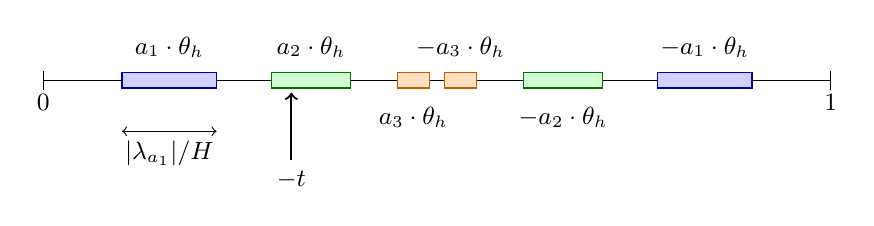
\begin{tikzpicture}[x=1cm,y=1cm,font=\small]
 \draw (0,0)--(10,0);
 \draw (0,-.12)--(0,.12) node[below=5pt] {$0$};
 \draw (10,-.12)--(10,.12) node[below=5pt] {$1$};
 \filldraw[fill=blue!18,draw=blue!65!black] (1,-.10) rectangle (2.2,.10);
 \filldraw[fill=blue!18,draw=blue!65!black] (7.8,-.10) rectangle (9,.10);
 \filldraw[fill=green!18,draw=green!45!black] (2.9,-.10) rectangle (3.9,.10);
 \filldraw[fill=green!18,draw=green!45!black] (6.1,-.10) rectangle (7.1,.10);
 \filldraw[fill=orange!25,draw=orange!75!black] (4.5,-.10) rectangle (4.9,.10);
 \filldraw[fill=orange!25,draw=orange!75!black] (5.1,-.10) rectangle (5.5,.10);
 \node at (1.6,.42) {$a_1\cdot\theta_h$};
 \node at (3.4,.42) {$a_2\cdot\theta_h$};
 \node at (4.7,-.47) {$a_3\cdot\theta_h$};
 \node at (5.3,.42) {$-a_3\cdot\theta_h$};
 \node at (6.6,-.47) {$-a_2\cdot\theta_h$};
 \node at (8.4,.42) {$-a_1\cdot\theta_h$};
 \draw[->,thick] (3.15,-1.02) node[below] {$-t$} -- (3.15,-.16);
 \draw[<->] (1,-.65)--(2.2,-.65)
    node[midway,below] {$|\lambda_{a_1}|/H$};
\end{tikzpicture}
\caption{Schematic signed intervals for one block, drawn in a representative
of $\T$.  Paired intervals have the same width and opposite centers.  The
construction packs the intervals for every block together.  Only an interval
containing $-t$ can give a nonzero stationary contribution at angle $t$;
the diagram illustrates this condition, not a particular packing produced
by the lemma.}
\label{fig:sampling-intervals}
\end{figure}

By \eqref{eq:sampling-coefficient-budget}, the modulus of the sole
possible leading contribution, including its Fourier coefficient, is at
most $K_\delta$.  Summing the errors over the fixed finite set of pairs
$(a,h)$ therefore gives
\begin{equation}\label{eq:sampling-uniform-maximum}
 \frac1{\sqrt N}\max_{t\in\T}
 \left|\sum_{k=0}^{N-1}X_{N,k}\e(kt)\right|
 \le K_\delta+o(1).
\end{equation}
The error tends to zero uniformly in $t$, with all construction data held
fixed.  We have obtained the desired maximum bound; it remains to show
that sampling retains the mean-square mass of $F$.

\paragraph{The mean-square mass.}
The block supports are disjoint, so products from different blocks vanish.
Within block $h$, a pair $a,a'\in\mathcal A$ contributes the coefficient
$c_a\overline{c_{a'}}$ times
\begin{equation}\label{eq:sampling-energy-term}
 \frac1N\sum_{k\in\Z}\chi_h(k/N)^2
 \e\!\left(k\beta+\frac{N\kappa}{2}(k/N-x_h^*)^2\right),
 \quad
 \beta=(a-a')\cdot\theta_h,\quad
 \kappa=\lambda_a-\lambda_{a'}.
\end{equation}
If $a=a'$, this is a Riemann sum with limit $\int\chi_h^2$.
If $\kappa\ne0$, Lemma~\ref{lem:sampling-poisson}, now with amplitude
$\chi_h^2$, shows that the sum with normalization $N^{-1/2}$ is bounded.
The additional factor $N^{-1/2}$ in \eqref{eq:sampling-energy-term}
therefore makes this contribution tend to zero.

The remaining case is $a\ne a'$ and $\kappa=0$.  It cannot be omitted:
the coefficient-spreading construction deliberately produces repeated
curvatures.  The centers of $I_{a,h}$ and $I_{a',h}$ are distinct modulo
one, so $\beta\notin\Z$.  Geometric summation gives
\[
 \left|\sum_{k=u}^{w}\e(k\beta)\right|
 \le\frac2{|1-\e(\beta)|}\qquad(u,w\in\Z,\ u\le w).
\]
Writing $\psi=\chi_h^2$, summation by parts consequently bounds
$\sum_k\psi(k/N)\e(k\beta)$ by a fixed constant times
$\norm{\psi}_\infty+\int|\psi'|$.  Indeed the discrete variation is at
most $\int|\psi'|$.  Division by $N$ again makes
\eqref{eq:sampling-energy-term} tend to zero.

\begin{samepage}
There are only finitely many pairs, so we may sum these limits.  Parseval
on the auxiliary torus gives
\begin{align}
 \lim_{N\to\infty}\frac1N\sum_{k=0}^{N-1}X_{N,k}^2
 &=\left(\sum_{h=1}^H\int\chi_h^2\right)
            \sum_{a\in\mathcal A}|c_a|^2
 \notag\\
 &=\left(\sum_{h=1}^H\int\chi_h^2\right)\norm{F}_2^2
 \notag\\
 &\ge(1-\delta)(1-3\delta)^2
   =1-7\delta+15\delta^2-9\delta^3
   \ge1-7\delta.\label{eq:sampling-energy-limit}
\end{align}
\end{samepage}
Together with \eqref{eq:sampling-uniform-maximum}, this proves
Proposition~\ref{prop:almost-signs}.
Every integer $N$ was allowed throughout.  In particular, neither the
packing prime nor the number of blocks imposes a divisibility condition
on $N$.
\end{proof}

\section{Rounding with a small defect mass}\label{sec:rounding}

We now prove Lemma~\ref{lem:rounding}.  Its input is a real coefficient
vector whose entries have absolute values close to one in total.  We round
this vector to signs while controlling its Fourier sum.  The small total
defect limits the number of coordinates that need attention at each scale.
Spencer's discrepancy method gives the required square-root cancellation
\cite{Spencer1985}.  Balister, Bollob\'as, Morris, Sahasrabudhe and Tiba
\cite[Sections~4--5]{BalisterEtAl2020} apply partial coloring to round
bounded Fourier coefficients to signs in their real Littlewood
construction.  Here we track the total defect to make the rounding loss
small relative to $\sqrt N$.  To specify the real-matrix input precisely, we derive
it from the arbitrary-vector partial-coloring theorem of Lovett and Meka
\cite[Theorem~4 in the cited preprint version]{LovettMeka2015}.

\subsection{A discrepancy bound for real matrices}

\begin{lemma}\label{lem:rounding-matrix}
There is an absolute constant $C_0$ such that, for integers $1\le s\le R$
and a real matrix $B\in[-1,1]^{R\times s}$, there is a vector
$\xi\in\{-1,1\}^s$ satisfying
\[
 \norm{B\xi}_\infty\le C_0\sqrt{s\log(2R/s)}.
\]
\end{lemma}

\begin{proof}
We first state the partial-coloring input in its vector form.  Given
$v_1,\ldots,v_R\in\R^u$, a starting point $x_0\in[-1,1]^u$, and
nonnegative numbers $c_1,\ldots,c_R$ such that
\[
 \sum_{i=1}^R\exp(-c_i^2/16)\le u/16,
\]
the theorem of Lovett and Meka gives, for every sufficiently small
$\eta>0$, a point $x\in[-1,1]^u$ with
\[
 |\langle v_i,x-x_0\rangle|\le c_i\norm{v_i}_2
 \quad(1\le i\le R),
 \qquad
 |x_k|\ge1-\eta\quad\text{for at least }u/2\text{ coordinates }k.
\]
Letting $\eta$ tend to zero and taking a convergent subsequence gives a
point with at least $\lceil u/2\rceil$ coordinates equal to signs and the
same discrepancy bounds.  Indeed, there are only finitely many choices
of these coordinates, and all the displayed inequalities are closed
under limits.

Start at zero in $[-1,1]^s$.  At a stage with $u$ coordinates not yet
equal to signs, restrict the rows of $B$ to those coordinates, take their
current values as $x_0$, and choose
\[
 c_i=4\sqrt{\log(16R/u)}\qquad(1\le i\le R).
\]
The threshold sum is exactly $u/16$, and every restricted row has
Euclidean norm at most $\sqrt u$.  Thus this step changes each row sum
by at most $4\sqrt{u\log(16R/u)}$ and fixes at least half the remaining
coordinates.  Leave the fixed coordinates unchanged and repeat.
Zero rows impose no restriction.  The process terminates with a sign
vector.

If $u_h$ is the number of remaining coordinates before step $h$, starting
with $h=0$, then $u_h\le2^{-h}s$.  The function
$u\log(16R/u)$ is increasing for $0<u\le R$.  With
$L=\log(16R/s)\ge\log16$, the sum of the row errors is therefore at most
\[
 \begin{aligned}
 4\sum_h\sqrt{u_h\log(16R/u_h)}
 &\le4\sqrt{sL}\sum_{h=0}^{\infty}2^{-h/2}
       \sqrt{1+\frac{h\log2}{L}}\\
 &\le4\sqrt{sL}\sum_{h=0}^{\infty}2^{-h/2}\sqrt{1+h/4}.
 \end{aligned}
\]
The last series converges, and $\log(16R/s)\le4\log(2R/s)$ for $s\le R$.
This proves the lemma with an absolute constant, including when $s=R$.
\end{proof}

\subsection{Dyadic rounding and the Fourier error}

The discrepancy estimate will be applied to real and imaginary Fourier
evaluations on a grid.  At each dyadic scale we can reverse all the
chosen signs without changing their discrepancy.  This permits rounding
without increasing the total defect mass, which is the source of the
improved error bound.

\begin{proof}[Proof of Lemma~\ref{lem:rounding}]
Let $X=(X_0,\ldots,X_{N-1})\in[-1,1]^N$ and
$\mu=\frac12\sum_k(1-|X_k|)$.  If $\mu=0$, every $X_k$ is already a
sign, and we take $\varepsilon_k=X_k$.  Suppose henceforth that
$0<\mu\le N/2$.  Set
\[
 \sigma_k=\begin{cases}1,&X_k\ge0,\\-1,&X_k<0,\end{cases}
 \qquad p_k=\frac{1-|X_k|}{2}.
\]
Then $X_k=\sigma_k(1-2p_k)$, $0\le p_k\le1/2$, and
$\sum_kp_k=\mu$.  In particular, this definition includes $X_k=0$.

Put $M=20N$ and $R=2M=40N$.  For the grid points
$t_\ell=\ell/M$, $0\le\ell<M$, define the real $R\times N$ matrix $A$ by
\[
 A_{2\ell,k}=\sigma_k\cos(2\pi kt_\ell),\qquad
 A_{2\ell+1,k}=\sigma_k\sin(2\pi kt_\ell)
 \quad(0\le k<N).
\]
Its entries belong to $[-1,1]$, and every selection of its columns has
at most $N\le R$ columns.

Choose an integer $J\ge1$ with $N2^{-J}\le1$, and first round down:
\[
 p^{(J)}_k=2^{-J}\lfloor2^Jp_k\rfloor.
\]
This does not increase the mass, and
\begin{equation}\label{eq:rounding-initial}
 \norm{A(p^{(J)}-p)}_\infty
 \le\sum_k|p^{(J)}_k-p_k|\le N2^{-J}\le1.
\end{equation}
We next construct $p^{(j-1)}$ from $p^{(j)}$, for $j=J,J-1,\ldots,1$,
preserving the two properties
\[
 p^{(j)}\in([0,1]\cap2^{-j}\Z)^N,
 \qquad \sum_kp^{(j)}_k\le\mu.
\]
Let $S_j$ be the set of coordinates for which $2^jp^{(j)}_k$ is odd,
and let $s_j=|S_j|$.  If $s_j=0$, no change is needed.  Otherwise apply
Lemma~\ref{lem:rounding-matrix} to the columns indexed by $S_j$, obtaining
signs $\xi_k$.  Replace all these signs by their negatives if necessary
so that $\sum_{k\in S_j}\xi_k\le0$, and define
\[
 p^{(j-1)}_k=
 \begin{cases}
 p^{(j)}_k+2^{-j}\xi_k,&k\in S_j,\\
 p^{(j)}_k,&k\notin S_j.
 \end{cases}
\]
An odd integer in $[0,2^j]$ lies between $1$ and $2^j-1$; adding either
sign therefore gives an even integer still in $[0,2^j]$.  Thus the
new vector belongs to $([0,1]\cap2^{-(j-1)}\Z)^N$.  Its mass does not
increase, and the simultaneous sign reversal has left the discrepancy
unchanged.  The step error is consequently at most
\begin{equation}\label{eq:rounding-step}
 \norm{A(p^{(j-1)}-p^{(j)})}_\infty
 \le C_0\,2^{-j}\sqrt{s_j\log(80N/s_j)}
 \qquad(s_j>0).
\end{equation}

Every coordinate in $S_j$ is at least $2^{-j}$, so the mass bound gives
\[
 s_j\le\min(N,2^j\mu).
\]
This is where the total defect enters the estimate.  Put
$U_j=2^j\mu$ and $L_\mu=\log(80N/\mu)$.  The function
$f(s)=s\log(80N/s)$ is increasing on $(0,N]$.  If $U_j\le N$, then
\[
 f(s_j)\le f(U_j)
 =U_j\log(80N/U_j)\le U_jL_\mu.
\]
If $U_j>N$, then, using $\mu\le N/2$,
\[
 f(s_j)\le N\log80\le U_jL_\mu.
\]
These estimates apply at every nonempty stage.  Summing
\eqref{eq:rounding-step} and \eqref{eq:rounding-initial} therefore gives,
for $p'=p^{(0)}\in\{0,1\}^N$,
\begin{equation}\label{eq:rounding-matrix-error}
 \begin{aligned}
 \norm{A(p'-p)}_\infty
 &\le1+C_0\sqrt{\mu L_\mu}\sum_{j=1}^{\infty}2^{-j/2}\\
 &=1+\frac{C_0}{\sqrt2-1}\sqrt{\mu\log(80N/\mu)}.
 \end{aligned}
\end{equation}
Empty stages contribute zero, without invoking the discrepancy bound
with no columns.

Now set $\varepsilon_k=\sigma_k(1-2p'_k)\in\{-1,1\}$ and define the
error polynomial
\[
 Q(z)=\sum_{k=0}^{N-1}(\varepsilon_k-X_k)z^k
     =-2\sum_{k=0}^{N-1}\sigma_k(p'_k-p_k)z^k.
\]
At a grid point, the real and imaginary parts of $-Q/2$ are
entries of $A(p'-p)$.  Hence
\begin{equation}\label{eq:rounding-grid}
 G:=\max_{0\le\ell<M}|Q(\e(t_\ell))|
 \le2\sqrt2\,\norm{A(p'-p)}_\infty.
\end{equation}
It remains to pass from this grid bound to the whole circle.  We apply
this step only to $Q$, the rounding error.

Write $S=\max_{|z|=1}|Q(z)|$.  If $Q=0$, there is nothing to prove.
Otherwise let $d\le N-1$ be its degree.  Applying the maximum principle
to $Q$ on the unit disk and to the reversed polynomial $z^dQ(1/z)$ gives
\[
 |Q(z)|\le S\max(1,|z|^d),
 \qquad
 \max_{|z|\le1+1/N}|Q(z)|\le \exp(1)S.
\]
Cauchy's estimate on the disk of radius $1/N$ centered at a point of
the unit circle yields $|Q'(z)|\le\exp(1)NS$ there.  Consequently
\[
 \left|\frac{d}{dt}Q(\e(t))\right|
 \le2\pi\exp(1)NS.
\]
Every point of $\T$ has circular distance at most $1/(2M)$ from the
grid.  Integrating this derivative along the shorter arc gives
\[
 S\le G+\frac{\pi\exp(1)}{20}S,
 \qquad
 S\le\frac{G}{1-\pi\exp(1)/20}.
\]
The denominator is positive.  Combining this inequality with
\eqref{eq:rounding-grid} and \eqref{eq:rounding-matrix-error} proves
Lemma~\ref{lem:rounding}, with an absolute constant.  The same argument
covers $N=1$, when the error polynomial is constant.
\end{proof}

\section{Flatness for every finite exponent}\label{sec:finite-flatness}
The maximum estimate and Parseval imply that normalized moduli converge
to one in $L^p$ for every fixed $0<p<\infty$. The same fourth-moment calculation
will give the merit-factor consequence in the next section.

\begin{corollary}\label{cor:finite-flatness}
There are Littlewood polynomials $P_N$ of every length $N$ such that,
for each fixed $0<p<\infty$,
\[
 \int_{\T}\left|\frac{|P_N(\e(t))|}{\sqrt N}-1\right|^p\,dt
 \longrightarrow0.
\]
\end{corollary}
\begin{proof}
Choose a minimizing polynomial at each length; the finite set of sign
vectors ensures that the minimum is attained. Put
$f_N(t)=|P_N(\e(t))|/\sqrt N$. Parseval and
Theorem~\ref{thm:main} give $\int f_N^2=1$ and
$\norm{f_N}_\infty=1+o(1)$. Hence
\[
 1\le\int f_N^4\le\norm{f_N}_\infty^2\int f_N^2=1+o(1),
 \qquad \int(f_N^2-1)^2\longrightarrow0.
\]
For $u\ge0$, $|u-1|^4\le|u^2-1|^2$, so
$\int|f_N-1|^4\to0$. For $p\le4$, the probability-space integral
inequality gives the assertion. For $p>4$, use the eventual uniform
bound on $|f_N-1|$ and the same fourth-moment convergence.
\end{proof}

\section{Binary merit factors and Morse shifts}\label{sec:merit-morse}
We now derive the autocorrelation and symbolic-dynamical consequences of
the maximum estimate. For a binary word
$A=(a_0,\ldots,a_{N-1})\in\{-1,1\}^N$, recall
\[
 P_A(z)=\sum_{j=0}^{N-1}a_jz^j,
 \qquad C_u(A)=\sum_{j=0}^{N-1-u}a_ja_{j+u}\quad(1\le u<N).
\]
For $N\ge2$, its merit factor is
$F(A)=N^2/(2\sum_{u=1}^{N-1}C_u(A)^2)$. The denominator is positive, since
$C_{N-1}(A)=a_0a_{N-1}\in\{-1,1\}$. Expanding $|P_A|^2$ on the unit
circle and applying Parseval with probability Haar measure gives
\begin{equation}\label{eq:merit-parseval}
 \norm{P_A}_4^4=N^2+2\sum_{u=1}^{N-1}C_u(A)^2,
 \qquad
 F(A)=\frac{N^2}{\norm{P_A}_4^4-N^2}.
\end{equation}
In the notation of Downarowicz--Lacroix,
$M_A=N^{-2}\sum_{u=1}^{N-1}C_u(A)^2$ and $F(A)=1/(2M_A)$
\cite[Definition~2 and Lemma~0]{DownarowiczLacroix1998}.

\begin{corollary}[All-length unbounded binary merit factors]\label{cor:merit}
For $N\ge2$, let
\[
 \mathcal F_N=\max_{A\in\{-1,1\}^N}F(A).
\]
Then
\[
 \lim_{N\to\infty}\mathcal F_N=+\infty,
\]
where the limit runs through all integer lengths. Equivalently, one can
choose a word $A_N\in\{-1,1\}^N$ for each $N\ge2$ such that
\[
 \sum_{u=1}^{N-1}C_u(A_N)^2=o(N^2).
\]
\end{corollary}
\begin{proof}
Choose $A_N$ so that $P_{A_N}$ attains the minimum defining $m_N$.
By \eqref{eq:merit-parseval}, Parseval, and the elementary fourth-moment
bound,
\[
 0<\frac1{F(A_N)}
 =\frac{\norm{P_{A_N}}_4^4}{N^2}-1
 \le\frac{\norm{P_{A_N}}_\infty^2\norm{P_{A_N}}_2^2}{N^2}-1
 =m_N^2-1\longrightarrow0.
\]
The last limit is Theorem~\ref{thm:main}. Thus $F(A_N)\to\infty$ and
$\mathcal F_N\ge F(A_N)$ has the same conclusion. The equivalence with
the autocorrelation formulation follows directly from the definition of
$F(A)$.
\end{proof}

This corollary refutes the bounded-merit-factor conjecture while retaining
the all-length quantifier of Theorem~\ref{thm:main}. It supplies no
quantitative rate of divergence.

For completeness, we specify the symbolic class in the next consequence.
For binary words $B$ and $C$ of lengths $b$ and $c$, respectively, their
product is defined by
\[
 (B\times C)(s+bt)=B(s)C(t)\qquad(0\le s<b,\ 0\le t<c).
\]
If each $B_j$ begins with $1$ and has length at least two, the products
$B_1\times\cdots\times B_j$ have a one-sided coordinatewise limit.
This limit admits a two-sided extension with the same finite words
\cite[Definition~3 and the following paragraph]{DownarowiczLacroix1998}.
The orbit closure $X\subset\{-1,1\}^{\Z}$ of such an extension, under
$Sx(n)=x(n+1)$, is a \emph{binary Morse shift}. This is the discrete-time
system called a Morse flow in that paper. Simple spectrum means that the
Koopman operator has a cyclic vector: the linear span of its integer iterates is
dense in the underlying $L^2$ space.

\begin{corollary}[Binary Morse spectral consequence]\label{cor:morse}
There is a binary Morse shift $(X,S)$ with a unique $S$-invariant Borel
probability measure $\mu$ for which the Koopman operator
$U_Sg=g\circ S$ on $L^2(X,\mu)$ has simple spectrum. For the
zero-coordinate function $f(x)=x(0)$, let $\sigma_f$ be the spectral
measure characterized by
\[
 \widehat{\sigma_f}(n):=\int_{\T}\e(nt)\,d\sigma_f(t)
 =\int_X f(x)f(S^n x)\,d\mu(x)\qquad(n\in\Z).
\]
Then $d\sigma_f=h\,dt$ for some $h\in L^2(\T)$ with $h\ge0$ almost
everywhere and $\int_{\T}h\,dt=1$. In particular, the absolutely
continuous spectral component is nonzero.
\end{corollary}
\begin{proof}
Corollary~\ref{cor:merit} supplies nontrivial finite binary words with
arbitrarily large merit factors. The forward construction in
\cite[Theorem~2 and its proof]{DownarowiczLacroix1998} therefore gives a
binary Morse shift with $\sum_{n=1}^{\infty}|\widehat{\sigma_f}(n)|^2<\infty$.
Its defining words have frequencies of both signs tending to $1/2$;
their Fact~1 gives unique ergodicity, and their Fact~2 gives simple
spectrum for that invariant measure.
Conjugate symmetry extends the square summability to $\Z$. Fourier
Plancherel and uniqueness of Fourier coefficients then give
$\sigma_f=h\,dt$ with $h\in L^2(\T)$. Positivity of $\sigma_f$ gives
$h\ge0$ almost everywhere, and
$\int h\,dt=\sigma_f(\T)=\norm{f}_2^2=1$.
\end{proof}

Here simplicity concerns the full Koopman operator, whereas absolute
continuity is asserted for the cyclic subspace generated by $f$; the
remaining spectral type is not identified. A different realization is
given in the companion manuscript \cite[Theorem~1.1]{OpenAIThreeTorus2026}:
it constructs a smooth volume-preserving diffeomorphism of $\T^3$ whose
Koopman operator has simple Lebesgue spectrum on the entire mean-zero
$L^2$ space. The present consequence instead concerns the constrained
class of binary Morse shifts.

\appendix
\section{Comparison with contrary flatness claims}\label{sec:concentration}

Corollary~\ref{cor:finite-flatness} conflicts with several stated
nonflatness results. We compare the precise versions listed in the
bibliography and examine the proposed obstructions. This discussion is
independent of the construction proving Theorem~\ref{thm:main}.

An earlier preprint of el Abdalaoui asserted nonexistence of
square-$L^2$-flat real Littlewood sequences
\cite[Theorem~3.3]{ElAbdalaoui2017}. Its definition fixes both endpoint
signs to $+1$ \cite[Equation~(2.1)]{ElAbdalaoui2017}. Changing at most
two endpoint signs of our length-$N$ polynomials costs at most
$4/\sqrt N$ in normalized uniform norm. Their normalized maxima still
tend to one, so the proof of Corollary~\ref{cor:finite-flatness} gives
square-$L^2$ flatness with this convention as well.

\subsection{The concentration constant and a neighborhood of zero}
Theorem~1 of \cite{ElAbdalaoui2025} claims that $L^2$-normalized real-sign
polynomial sequences cannot be $L^{2p}$-flat for integers $p>1$. This conflicts with
Corollary~\ref{cor:finite-flatness}, even though our maximum estimate
supplies no uniform lower bound. The final inference in the cited proof
uses a concentration constant with a different quantifier order from
the one needed there.

To see the distinction, let $\mathcal I$ be the nonzero analytic
idempotent trigonometric polynomials
\[
 I(t)=\sum_{k\in E_0}\e(kt),
 \qquad \varnothing\ne E_0\subset\Z_{\ge0}\text{ finite}.
\]
For $\alpha>0$ and a measurable set $E\subset\T$, define
\[
 B_\alpha(E)=\sup_{I\in\mathcal I}
      \frac{\int_E|I(t)|^\alpha\,dt}{\int_{\T}|I(t)|^\alpha\,dt}.
\]
The concentration level of Bonami--R\'ev\'esz is
\cite[Definitions 1--2]{BonamiRevesz2008}
\begin{equation}\label{eq:concentration-infimum}
 c_\alpha=\inf_{\substack{E\text{ symmetric, open}\\E\ne\varnothing}}
                B_\alpha(E).
\end{equation}
Indeed every number strictly smaller than the infimum is a concentration
guarantee for each such $E$, and every uniform guarantee is no larger
than the infimum. Thus an upper bound on $c_\alpha$ does not give that
upper bound on $B_\alpha(E)$ for a prescribed $E$.

For completeness, the particular sets used in the contrary inference
have optimal concentration equal to one. Suppose $E$ contains the
neighborhood $(-d,d)$ of zero, where $0<d<1/2$, and put
$D_q(t)=\sum_{k=0}^{q-1}\e(kt)$. The geometric-series formula gives
\[
 |D_q(t)|\le\frac1{\sin(\pi d)}\quad(t\notin E).
\]
For $|t|\le1/(2q)$, the same formula and
$\sin x\ge2x/\pi$ on $[0,\pi/2]$ give
$|D_q(t)|\ge2q/\pi$. Consequently, for $\alpha>1$,
\begin{align*}
 \int_{\T\setminus E}|D_q|^\alpha&\le\sin(\pi d)^{-\alpha},\\
 \int_{\T}|D_q|^\alpha&\ge(2/\pi)^\alpha q^{\alpha-1}.
\end{align*}
Their ratio tends to zero, proving $B_\alpha(E)=1$. Bonami--R\'ev\'esz
also explicitly distinguish full concentration at zero from the uniform
concentration level \cite[Theorem 7 and Proposition 9]{BonamiRevesz2008}.

Under its assumed flatness, Equation~(27) of \cite{ElAbdalaoui2025}
gives concentration tending to
one in each fixed neighborhood of zero. This is compatible with
\eqref{eq:concentration-infimum}; it does not contradict the cited upper
bound $c_{2p}\le1/2$. Multiplicative normalization cancels in the ratio.
Even restricting supports to $\{0,\ldots,q-1\}$ with density tending to
$1/2$ does not give the required cap: use $D_{\lfloor q/2\rfloor}$.
This explains the failure of that specific concluding inference.

\subsection{A later weighted assertion}
A separate preprint \cite[Theorem 1]{ElAbdalaoui2025Generalization}
asserts a nonflatness criterion for fixed real coefficients $a_j$ and
unimodular multipliers. Its hypothesis is
\begin{equation}\label{eq:weighted-hypothesis}
 \sum_{j=1}^n a_j^2\le\frac K{n^2}\sum_{j=1}^n j^2a_j^2,
\end{equation}
and its polynomial is normalized by $(\sum_{j=1}^n a_j^2)^{1/2}$.
Without any restriction preventing a dominant coefficient, this
criterion is false.

Take $a_j=2^{j^2}$ and all unimodular multipliers equal to one. Let
$S_n=\sum_{j=1}^n a_j^2$. For $n\ge2$,
\[
 \frac{\sum_{j<n}a_j^2}{a_n^2}
 \le(n-1)2^{-4n+2}\le1.
\]
It follows, also at $n=1$, that
\[
 S_n\le2a_n^2\le\frac2{n^2}\sum_{j=1}^n j^2a_j^2.
\]
Thus \eqref{eq:weighted-hypothesis} holds with $K=2$. On the other hand,
\[
 \frac{\sum_{j<n}a_j}{a_n}\le(n-1)2^{-2n+1}\longrightarrow0,
 \qquad \frac{S_n}{a_n^2}\longrightarrow1.
\]
Uniformly for $|z|=1$, therefore,
\[
 \left|\frac{\sum_{j=1}^n a_jz^j}{\sqrt{S_n}}-z^n\right|
 \le\frac{\sum_{j<n}a_j}{\sqrt{S_n}}
       +\left|\frac{a_n}{\sqrt{S_n}}-1\right|\longrightarrow0.
\]
The normalized moduli converge uniformly to one. This example concerns
weighted coefficients, not signs.

The proof of Corollary~3 in
\cite{ElAbdalaoui2025Generalization} displays a signed-modulus identity
for values at $|z|=|z'|=1$.
Even reading its repeated second argument as the intended $z'$, the
asserted form
\[
 |P(z)-P(z')|=\sigma|P(z)|+\tau|P(z')|,
 \qquad \sigma,\tau\in\{-1,1\},
\]
is false. For $P(z)=1+z$, $z=1$ and $z'=i$, the left side is $\sqrt2$,
whereas no value $\pm2\pm\sqrt2$ equals $\sqrt2$.
These observations identify defects in the proposed obstructions;
the real-sign assertion of Theorem~\ref{thm:main} rests on the
construction and rounding proof above.

\bibliographystyle{plain}
\bibliography{refs}
\end{document}
